% !TeX program = pdflatex
% ==========================================================================
%  PACDIS -- two-column manuscript draft (Elsevier elsarticle, 5p layout)
%
%  PAQC is the primary contribution; simplified CDIS supports batch selection.
%  Implementation: REMO_UniformMix_Pruned_Weighted_Lambdat030_NoBatchDist.
%  Original-parameter checkpoint: paper-original-params-20260914.
%  Established components are cited where they enter the framework.
%
%  Layout notes:
%    * elsarticle option "5p" is Elsevier's final two-column journal layout
%      (textwidth 522pt, columnsep 18pt => 252pt columns) and it loads
%      fleqn.clo, so displayed equations are flush left.
%    * Wide displays are broken with split/multline and wide floats use the
%      starred environments (table*, algorithm*) to span both columns.
%      Line breaking and float placement are adapted to the column width; the
%      wording and the mathematics are not affected by it.
%    * For the double-spaced single-column referee version, swap the class
%      options for [preprint,review,12pt].
% ==========================================================================
\documentclass[final,5p,times,twocolumn]{elsarticle}

\usepackage{amsmath,amssymb,amsthm}
\usepackage{bm}
\usepackage{booktabs}
\usepackage{algorithm}
\usepackage{algpseudocode}
\usepackage{enumitem}
\usepackage{xcolor}
\usepackage{colortbl}
\usepackage{placeins}
\usepackage[hidelinks]{hyperref}

% graphicx is already loaded by elsarticle.cls


% Narrow columns: allow slightly looser lines before an overfull box.
\tolerance=1200
\emergencystretch=1em

% Pseudo-code is set one size down so that the wider \State lines fit a column.
\usepackage{etoolbox}
\AtBeginEnvironment{algorithmic}{\footnotesize}
\algrenewcommand{\algorithmicrequire}{\textbf{Input:}}
\algrenewcommand{\algorithmicensure}{\textbf{Output:}}

\newcommand{\vf}{\mathbf{f}}
\newcommand{\vx}{\mathbf{x}}
\newcommand{\vv}{\mathbf{v}}
\newcommand{\vu}{\mathbf{u}}
\newcommand{\vw}{\mathbf{w}}
\newcommand{\vr}{\mathbf{r}}
\newcommand{\vz}{\mathbf{z}}
\newcommand{\TODO}[1]{\textcolor{red}{[TODO: #1]}}

%% Uncomment and fill in for a preprint that names its target journal.
%% \journal{Information Sciences}

\begin{document}

%% Float placement. The wide ablation/sensitivity tables and the convergence
%% figure are close to a full page each; with the defaults LaTeX refuses to
%% put a table and a figure on the same page and drops each onto its own
%% float page, which leaves half-empty pages. These thresholds let the pair
%% share a page while still reserving room for running text. They must be set
%% after \begin{document}: elsarticle resets them at the start of the body.
\renewcommand{\topfraction}{0.9}
\renewcommand{\bottomfraction}{0.6}
\renewcommand{\textfraction}{0.02}
\renewcommand{\floatpagefraction}{0.7}


\begin{frontmatter}

\title{PBI-Assisted Quality Classification and Criterion-Diversified Infill Selection
for Expensive Many-Objective Optimization}

%% Author block. Replace the placeholders and add \corref/\ead as needed:
%% \author[inst1]{Given Name Surname\corref{cor1}}
%% \ead{name@example.edu}
%% \cortext[cor1]{Corresponding author.}
\author{\TODO{author list}}

\affiliation{organization={Department, University},
            addressline={Street},
            city={City},
            postcode={000000},
            state={Province},
            country={Country}}

\begin{abstract}
\TODO{Use the challenge--contribution structure. State the two concrete gaps:
REMO forms training groups using a small set of representatives selected through
RSEA's two-dimensional radial projection. These representatives may not fully
reflect the current nondominated distribution in the original objective space,
and relation scores alone leave the use of prediction ambiguity and indicator
information in candidate selection unspecified. Introduce PACDIS with PBI-assisted
quality classification (PAQC) and criterion-diversified infill selection (CDIS).
PAQC constructs adaptive directions directly from the current nondominated
objective vectors and uses PBI-based directional quality information to supplement
representative-based positive-group construction. CDIS provides a supporting
batch-selection strategy. Lead the results
with the strongest verified algorithm-level IGD$^+$ comparison in the tested
many-objective settings. Then give one concise mechanism finding about group
composition or candidate-batch utility. Keep detailed overlap statistics and
componentwise tests in the experimental section.}
\end{abstract}

\begin{keyword}
expensive many-objective optimization \sep surrogate-assisted evolutionary
algorithm \sep relation learning \sep penalty-based boundary intersection \sep
infill selection
\end{keyword}

\end{frontmatter}

\section{Introduction}
\label{sec:intro}

\TODO{Use a four-move opening: expensive many-objective relation learning; the
potential loss of high-dimensional distribution information when grouping relies
on representatives selected through two-dimensional radial projection, and
the use of prediction ambiguity and indicator information in candidate selection; PAQC as the
primary contribution and CDIS as its supporting selection strategy; and algorithm-level performance followed by evidence explaining
group construction and candidate selection. Present the two mechanisms as
complementary design roles in one algorithm. Do not lead with selection-overlap
statistics or imply that the relation network learns a within-group ordering.}

REMO~\cite{ref:remo} constructs its training groups from a small set of
representative solutions selected using the radial-space mechanism of
RSEA~\cite{ref:rsea}. RSEA projects high-dimensional objective vectors into a
two-dimensional radial space, where grid division supports efficient selection.
Its authors acknowledge that this reduction loses curvature information and
design a selection strategy to mitigate its impact~\cite{ref:rsea}.
For representative-based grouping, this motivates a further question: do the
directions induced by the selected representatives sufficiently reflect the
current nondominated distribution in the original objective space?

The primary contribution is PBI-assisted quality classification (PAQC).
PAQC supplements REMO's representative-based grouping with PBI-based quality
information from directions constructed directly from current nondominated
objective vectors. These directions supply distribution information from the
original objective space without passing through the two-dimensional radial grid.
PAQC combines this directional quality information with the original binary
labels to construct the positive training group, retaining REMO's three-class
relation-learning scheme~\cite{ref:remo}.
To support the use of these predictions,
criterion-diversified infill selection (CDIS) provides two batch-selection
criteria within an explicit evaluation cap. One ranks candidates by relation
quality and prediction ambiguity after a quality screen; the other
reranks a relation-screened subset using a predicted indicator. This supporting
strategy uses a fixed ambiguity reward in the first branch and predicted
indicator values in the second branch.

\section{Related Work}
\label{sec:related}

\subsection{Surrogate-Assisted Expensive Multi-/Many-Objective Optimization}
\label{sec:related:saea}
\TODO{Kriging/RBF-based SAEAs, their scalability limit in $M$, and why
regression on every objective becomes unattractive when $M$ grows.}

\subsection{Relation Learning for Expensive Optimization}
\label{sec:related:relation}
\TODO{REMO and the pairwise-comparison SAEA line; compare how each method forms
training groups or pairwise labels, then position the present work as
group construction that supplements directions induced by radially selected
representatives with directions obtained directly from the current nondominated
set. Explain how directional quality information and the original binary labels jointly
determine training-group membership.}

\subsection{Quality Assessment and Candidate Selection}
\label{sec:related:selection}
\TODO{Indicator-based assessment (SDE, $L_p$ shape estimation, PIEA), radial
representative selection (RSEA), and infill/candidate selection rules.}

RSEA uses radial projection and adaptive grids for selection, with both
crowding and convergence considered to address the effects of curvature
information loss~\cite{ref:rsea}. PAQC retains this representative-selection
mechanism and supplements its grouping signal with a separate assessment in
the original objective space. The distinction concerns the source of directional
information, rather than the binary form of the original labels alone.

\section{The Proposed PACDIS}
\label{sec:method}

Relation-based surrogate-assisted evolutionary algorithms replace multi-output
regression by a classifier that predicts the relative quality of a pair of
solutions~\cite{ref:remo}. Two interfaces then decide what such an algorithm
can learn and how much its predictions cost: the rule that turns the evaluated
population into supervision labels, and the rule that turns the surrogate
scores of a large candidate pool into a small batch of expensive evaluations.
We propose PACDIS, a surrogate-assisted many-objective evolutionary
algorithm centred on improving the supervision interface through PAQC,
with CDIS providing a supporting expensive-evaluation selection strategy.
\emph{PBI-assisted quality classification} (PAQC) augments the
representative-based grouping of REMO~\cite{ref:remo} with PBI-based quality
information from directions constructed directly from the current nondominated
set. This additional source enriches the distribution information available for
relation-group construction. PAQC fuses the two signals to determine which
solutions enter the positive training group.
\emph{Criterion-diversified infill selection} (CDIS) retains relation-guided
candidate generation but uses either indicator-based reranking or
ambiguity-rewarded ranking to choose the final expensive-evaluation
batch. Established relation learning, indicator assessment and environmental
selection modules provide the host algorithm; the two proposed mechanisms
change how its training groups are formed and how its surrogate scores are used.

\subsection{Overall Framework}
\label{sec:method:framework}

We consider the expensive many-objective problem
\begin{equation}
\min_{\vx\in\Omega}\;
\vf(\vx)=\bigl[f_1(\vx),\ldots,f_M(\vx)\bigr],
\qquad
\Omega\subseteq\mathbb{R}^{D},
\label{eq:problem}
\end{equation}
in which every evaluation of $\vf$ is expensive, so the number of real function
evaluations is limited to a budget $FE_{\max}$. Let $FE$ be the number of
evaluations consumed so far and $t=FE/FE_{\max}\in[0,1]$ the evaluation
progress, which controls the hybrid score in PAQC.

PACDIS evaluates a Latin hypercube design of $N_{\mathrm{init}}$ solutions,
stores them in an archive $\mathcal{A}_{\mathrm{rc}}$, and then repeats five
steps until the budget is exhausted. (i)~The current population $\mathcal{P}$
is divided into a positive group and a non-positive group by
PAQC, which also returns the set $\mathcal{R}$ of
representative solutions reused later as an additional mating pool.
(ii)~Ordered pairs are generated from the two groups and a three-class relation
network is trained using the resulting ordered group labels.
(iii)~An indicator value is computed for each solution in $\mathcal{P}$ and an
RBF-SVR model is fitted from decision vectors to those values.
(iv)~One of the two selection modes is drawn, a relation-guided inner search
accumulates candidates under that mode, and a batch of at most $n_{\max}$ candidates is
returned. (v)~The batch is evaluated, appended to
$\mathcal{A}_{\mathrm{rc}}$, and the next population is obtained by the
radial-grid environmental selection of RSEA~\cite{ref:rsea} over the whole
archive.

Algorithm~\ref{alg:framework} states the procedure; its grouping and candidate
selection steps are detailed in Algorithms~\ref{alg:paqc}
and~\ref{alg:cdis}, respectively. The initial design satisfies
$2\leq N_{\mathrm{init}}\leq FE_{\max}$, and $N$ is the target population size
for environmental selection. The relation surrogate $\mathcal{M}_R$ includes
the group references and input normalisation needed for prediction, while
$\mathcal{M}_I$ denotes the indicator surrogate when available. The controls
are shared by the three procedures.
All expensive evaluations
after initialisation are consumed in step~(v), so both proposed mechanisms operate on already
evaluated data and surrogate predictions only, and neither changes the total
number of real evaluations. The two interfaces stay separate: grouping
decides \emph{what the classifier is asked to learn}, candidate selection
decides \emph{how its scores are spent}.

Figure~\ref{fig:framework} shows the evaluation loop and expands CDIS into its
relation-guided candidate search and criterion-dependent infill branches.
\begin{figure*}[t]
  \centering
  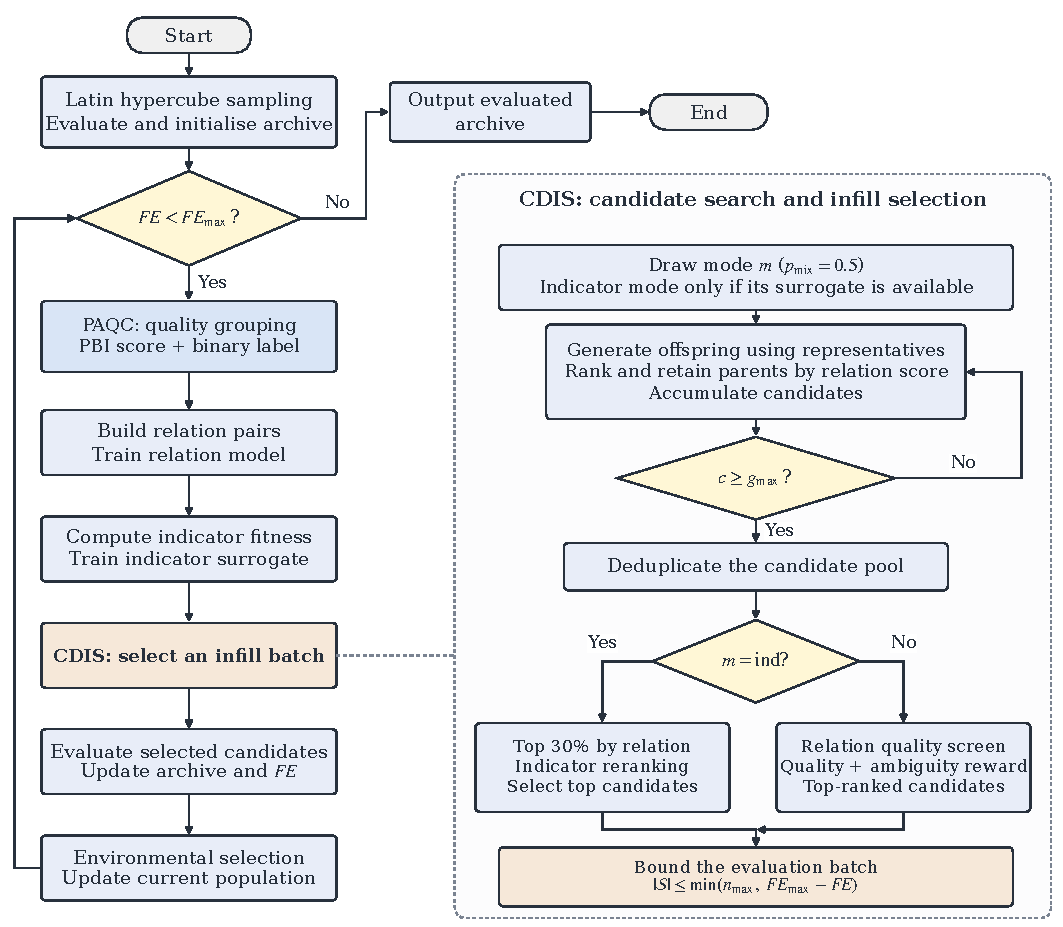
\includegraphics[width=0.98\textwidth]{figures/fig_framework.pdf}
  \caption{Overall framework of PACDIS. PAQC constructs the
  supervision groups for relation learning, and CDIS
  allocates a bounded batch of expensive evaluations. The representatives also
  enter the mating pool (dashed arrow). The indicator surrogate is trained on
  the current evaluated population. Newly evaluated solutions enter the archive,
  from which environmental selection constructs the next population.
  \label{fig:framework}}
\end{figure*}


\begin{algorithm}[t]
\caption{PACDIS}
\label{alg:framework}
\begin{algorithmic}[1]
\Require problem $(\Omega,\vf)$, budget $FE_{\max}$, initial size
         $N_{\mathrm{init}}$, population size $N$
\Ensure archive $\mathcal{A}_{\mathrm{rc}}$ of evaluated solutions
\State $\mathcal{P}\gets N_{\mathrm{init}}$ solutions sampled by Latin hypercube design
\State Evaluate $\mathcal{P}$; $FE\gets N_{\mathrm{init}}$
\State $\mathcal{A}_{\mathrm{rc}}\gets\mathcal{P}$
\While{$FE<FE_{\max}$}
  \State $t\gets FE/FE_{\max}$
  \State $(\mathcal{C}_1,\mathcal{C}_2,\mathcal{R})\gets$
         \Call{PBIQualityClassification}{$\mathcal{P},t$}
  \State Build ordered relation pairs from $\mathcal{C}_1,\mathcal{C}_2$ by
         \eqref{eq:pairlabel}
  \State Train the relation surrogate $\mathcal{M}_R$
  \State Train the indicator surrogate $\mathcal{M}_I$ on $\mathcal{P}$
  \State Draw an exploration or indicator mode $m$
  \State $\mathcal{S}\gets$ \Call{CDIS}{$\mathcal{P},\mathcal{R},\mathcal{M}_R,\mathcal{M}_I,m$}
  \State Evaluate $\mathcal{S}$ and append it to $\mathcal{A}_{\mathrm{rc}}$
  \State $FE\gets FE+|\mathcal{S}|$
  \State $\mathcal{P}\gets$ \Call{EnvSelect}{$\mathcal{A}_{\mathrm{rc}},N$}
\EndWhile
\State \Return $\mathcal{A}_{\mathrm{rc}}$
\end{algorithmic}
\end{algorithm}

\subsection{PBI-Assisted Quality Classification (PAQC)}
\label{sec:method:paqc}

Relation learning requires training groups that reflect the quality of evaluated
solutions. REMO~\cite{ref:remo} derives its grouping signal from a small set of
representatives selected through RSEA's two-dimensional radial grid~\cite{ref:rsea}.
These representatives retain their original objective vectors, but the projected
distribution guides their selection. This sparse summary may not fully reflect
the directional distribution of the current nondominated solutions in the
original many-objective space.

PAQC supplements this representative-based grouping signal with quality
information derived directly from the current nondominated solutions.
It constructs reference directions from their original objective vectors,
bypassing radial-grid representative selection, and uses PBI to assess evaluated
solutions along these directions. A stage-dependent fusion combines the
directional quality information with the original representative-based labels.
The highest-ranked fraction forms the positive training group, and the remaining
solutions form its complement. PAQC thus retains REMO's representative-based
signal while adding another information source for relation-group construction.

Figure~\ref{fig:paqc-mechanism} provides a geometric overview of these two
signals and their roles in grouping.

\begin{figure}[!t]
\centering
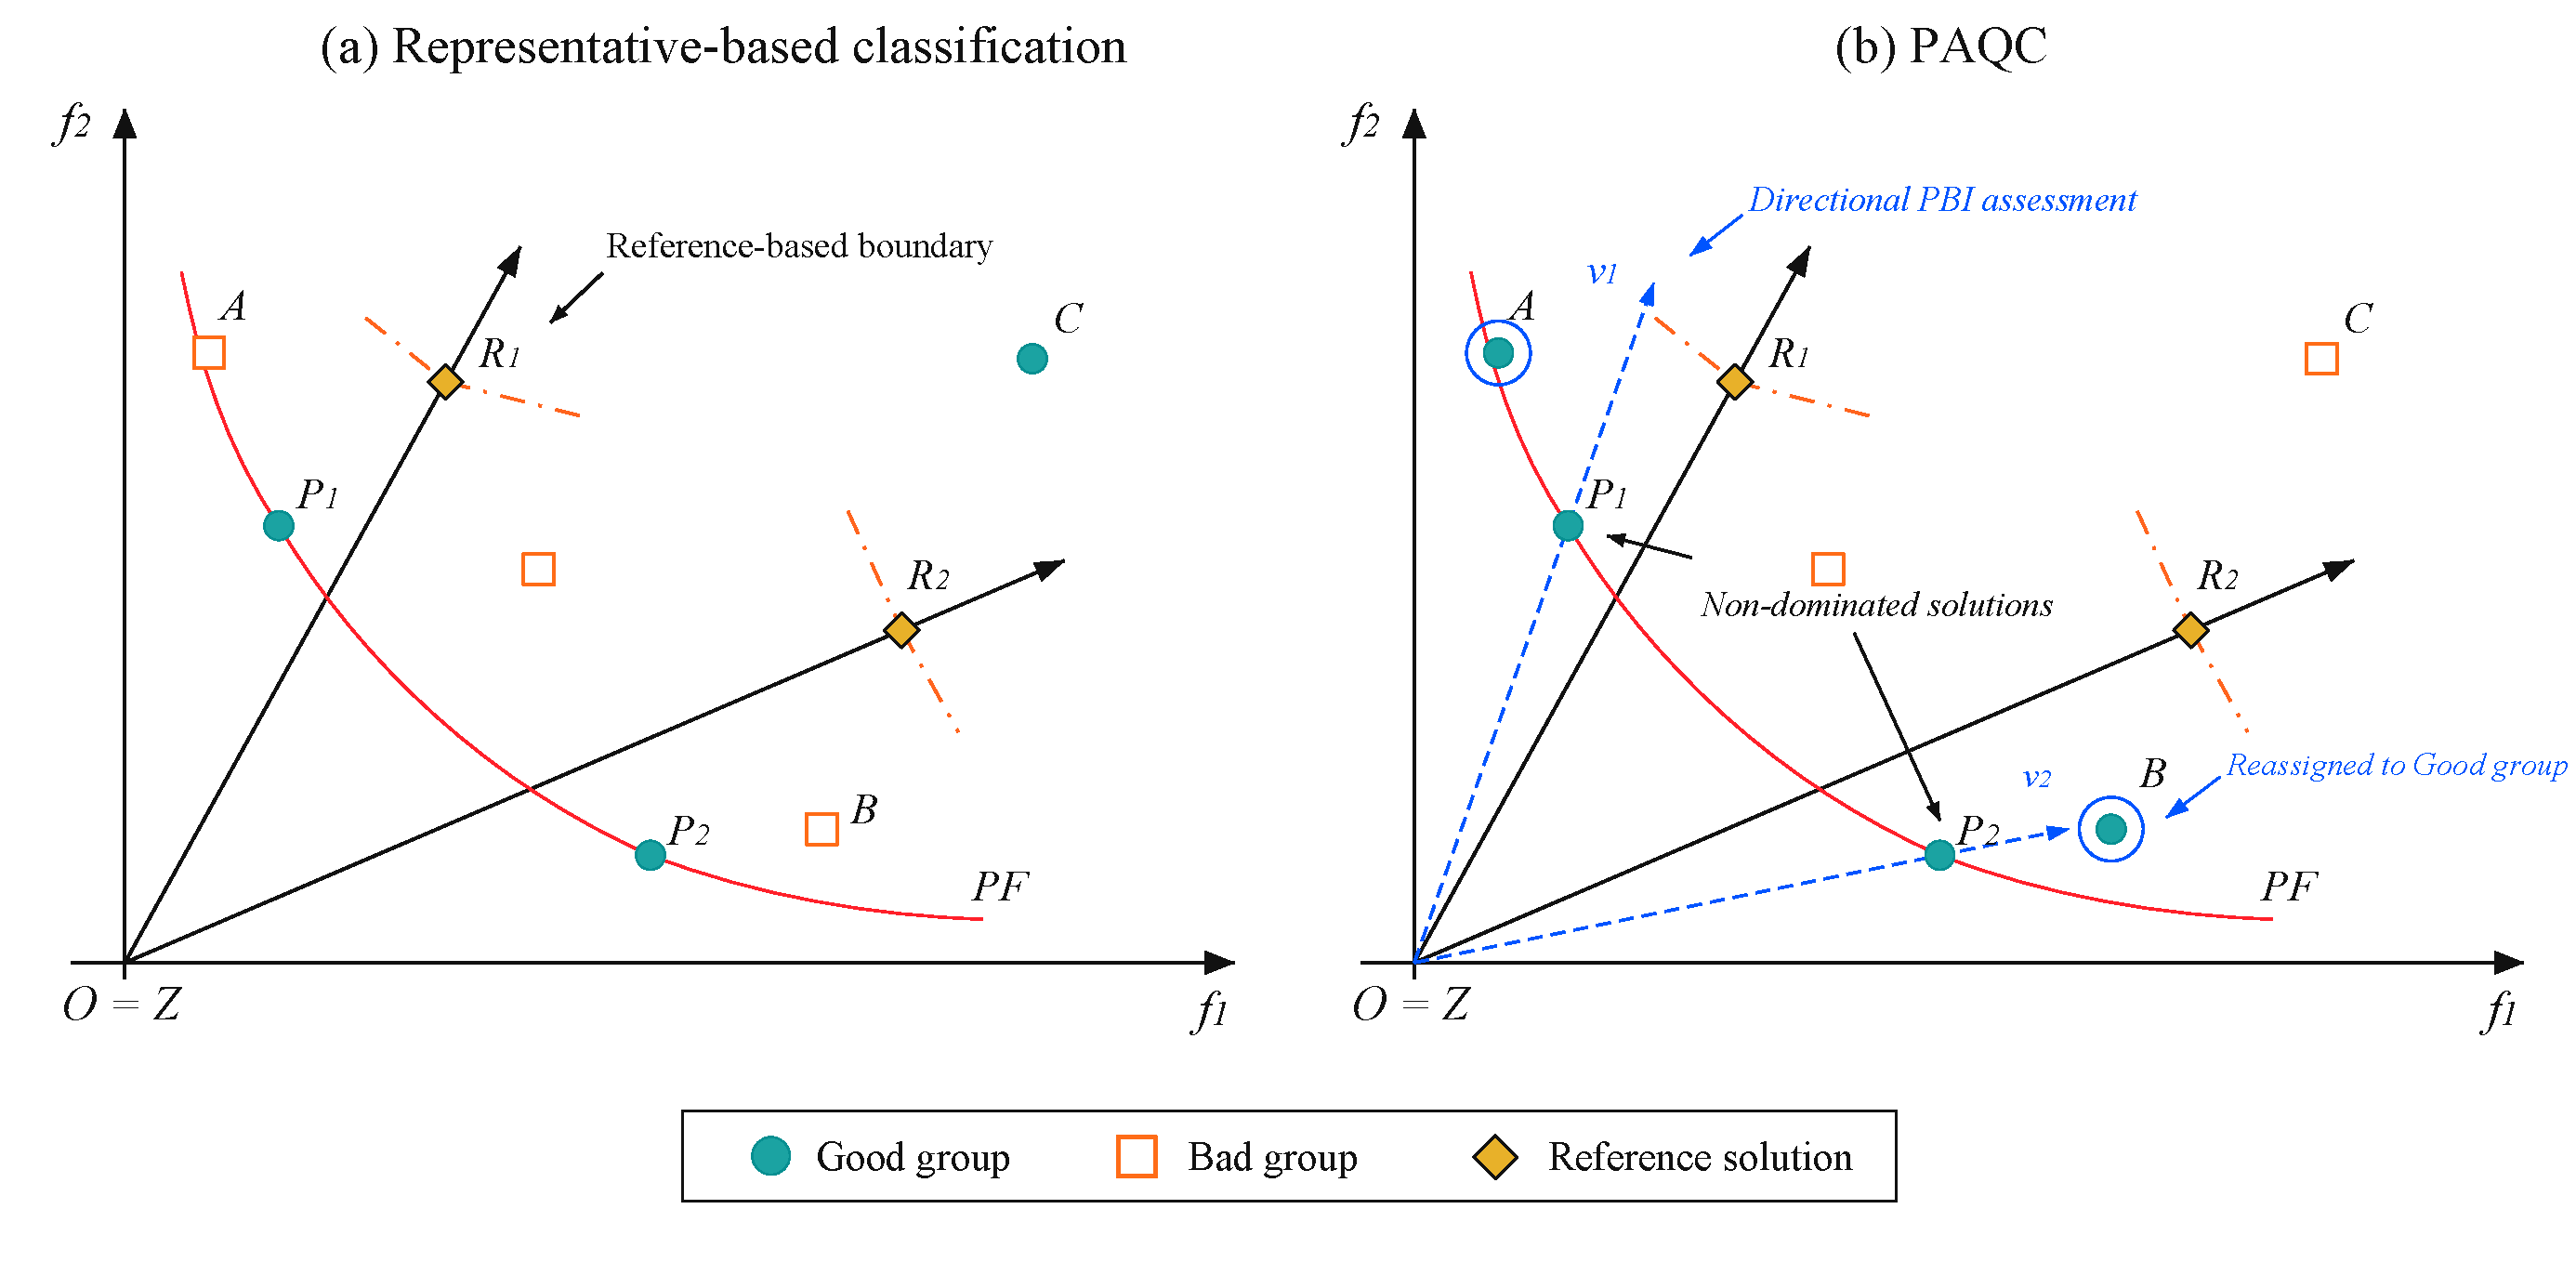
\includegraphics[width=\columnwidth]{figures/paqc_reference_edit/paqc_geometry_v5_editable.pdf}
\caption{Conceptual illustration of representative-based classification and
PAQC. Black rays connect the ideal point $Z$ to representative solutions, and
orange dash-dotted segments indicate local classification thresholds. Blue
dashed rays show directions constructed from nondominated solutions $P_1$ and
$P_2$. In (a), ``Good group'' and ``Bad group'' denote the binary labels
$L_i=1$ and $L_i=0$; in (b), they denote $\mathcal{C}_1$ and
$\mathcal{C}_2$, respectively. Blue rings highlight the reassignment of $A$
and $B$. The PF is an external reference only. Selected solutions and schematic
boundaries are shown, rather than a complete population or a numerically
evaluated example. Geometric presentation adapted from REMO~\cite{ref:remo}.}
\label{fig:paqc-mechanism}
\end{figure}

For PAQC, $\mathcal{P}=\{(\vx_i,\vf_i)\}_{i=1}^{N}$ is the
current population, with $N=|\mathcal{P}|$, and $\vz^{*}=\min_i\vf_i$ the component-wise population
minimum, taken as the ideal point.

\subsubsection{Quality Assessment Using Nondominated-Derived Directions}
\label{sec:method:paqc:cont}

The current nondominated solutions provide the additional directional information.
Let $\{\vf^{(j)}\}_{j=1}^{n_{\mathrm{ND}}}$ denote the objective vectors of
the first nondominated front. PAQC normalises these original objective vectors
to construct the reference-direction set $\mathcal{V}=\{\vv_j\}$:
\begin{equation}
\mathcal{V}=\Bigl\{\vf^{(j)}\big/\bigl\|\vf^{(j)}\bigr\|_2
\;\Bigm|\;j=1,\ldots,n_{\mathrm{ND}}\Bigr\}.
\label{eq:direction}
\end{equation}
The number and orientations of these directions follow the current nondominated
distribution in the original objective space. This construction uses the
nondominated vectors directly, without radial-grid representative selection.
When the adaptive construction is not applicable, PAQC uses uniformly distributed
reference directions as a fallback. This includes $M\leq3$, $N<50$, too few
nondominated solutions, or a degenerate objective range in the nondominated set.

Each objective vector is associated with the direction of largest cosine
similarity, $a(i)=\arg\max_j
\vf_i^{\mathsf T}\vv_j/(\|\vf_i\|_2\|\vv_j\|_2)$, and the conventional
PBI value~\cite{ref:moead} along that direction is
\begin{equation}
\begin{aligned}
d_{1,i}&=(\vf_i-\vz^{*})^{\mathsf T}\vv_{a(i)}\big/\|\vv_{a(i)}\|_2,\\
d_{2,i}&=\bigl\|(\vf_i-\vz^{*})
        -d_{1,i}\,\vv_{a(i)}/\|\vv_{a(i)}\|_2\bigr\|_2,\\
g_i^{\mathrm{PBI}}&=d_{1,i}+\theta\,d_{2,i},
\end{aligned}
\label{eq:pbi}
\end{equation}
with penalty $\theta$. PAQC maps this PBI value to a bounded quality signal:
\begin{equation}
S_i=\frac{1}{1+g_i^{\mathrm{PBI}}}\in(0,1],
\label{eq:score-cont}
\end{equation}
so a larger $S_i$ indicates a smaller PBI value along the associated direction.
This transformation expresses the directional assessment as a bounded signal
for fusion with the representative-based label during group construction.

\subsubsection{Representative-Based Grouping Signal}
\label{sec:method:paqc:coarse}

PAQC retains the representative-based grouping signal used in REMO~\cite{ref:remo}.
RSEA's radial-grid selection~\cite{ref:rsea} supplies a small set
$\mathcal{R}\subset\mathcal{P}$ of $k$ representative solutions from the current
population. These representatives induce the original binary grouping signal. The
representatives are evaluated solutions that act as dynamic, population-derived
reference points. We set the requested representative count to
$k=\lceil1.5M\rceil$ in the considered experiments; the implementation bounds
are given in Section~\ref{sec:exp:settings}.

Given $\mathcal{R}$, the binary group label applies the PBI partition of
REMO~\cite{ref:remo} with the representatives as reference points. Every
solution is associated with the representative $\vr_{b(i)}$ of largest cosine
similarity, the associated direction is
$\vw_{b(i)}=(\vr_{b(i)}-\vz^{*})/\|\vr_{b(i)}-\vz^{*}\|_2$, the two distances
$\hat d_{1,i},\hat d_{2,i}$ are formed as in \eqref{eq:pbi} with
$\vv_{a(i)}$ replaced by $\vw_{b(i)}$, and the binary label is
\begin{equation}
L_i=\mathbb{I}\!\left[
\frac{\hat d_{1,i}+\delta\,\hat d_{2,i}}
     {\|\vr_{b(i)}-\vz^{*}\|_2}\leq1\right]\in\{0,1\}.
\label{eq:label-bin}
\end{equation}
Normalising by $\|\vr_{b(i)}-\vz^{*}\|_2$ makes the associated representative
itself the threshold, so $L_i$ records on which side of the surface through that
representative a solution lies. Following REMO, the class-balance variable
$\delta$ is adjusted by bounded bisection so that the boundary maintains useful
occupancy on both sides across changing population states.

\subsubsection{Complementary-Signal Fusion for Positive-Group Construction}
\label{sec:method:paqc:hybrid}

The representative-based label describes membership relative to the selected
reference solutions, while the nondominated-derived directions supply additional
quality information from the original objective space. PAQC combines these two
information sources with a weight that follows consumption of the expensive budget. With
$t=FE/FE_{\max}$ and $\alpha_t=1-t$, the hybrid quality score of solution $i$ is
\begin{equation}
H_i=\alpha_t S_i+(1-\alpha_t)L_i ,
\qquad
\alpha_t=1-t ,
\label{eq:fuse}
\end{equation}
and the positive group collects the highest-ranked fraction $r_g$ of the
population,
\begin{equation}
\mathcal{C}_1=\bigl\{\vx_i\;\big|\;
\operatorname{rank}_{\downarrow}(H_i)\leq\lceil r_gN\rceil\bigr\},
\qquad
\mathcal{C}_2=\mathcal{P}\setminus\mathcal{C}_1 .
\label{eq:group}
\end{equation}
With $r_g<1/2$ the non-positive group $\mathcal{C}_2$ provides a broad contrast
set, while the compact positive group concentrates pairwise supervision on the
highest-priority portion of the population.

Figure~\ref{fig:paqc-mechanism} illustrates the distinct roles of the two PBI
signals. In panel~(a), the representatives $R_1$ and $R_2$ define the local
thresholds used to obtain $L_i$. In panel~(b), the nondominated solutions
$P_1$ and $P_2$ supply the adaptive directions $\vv_1$ and $\vv_2$ through
\eqref{eq:direction}; these directions provide an additional directional
assessment through $S_i$, rather than directly defining a new classification
boundary. The reassignment of $A$ and $B$ to the positive
group and of $C$ to its complement schematically depicts how the additional
directional information can change selection priorities through
\eqref{eq:fuse}--\eqref{eq:group}. PAQC therefore modifies the ranking used to form
the groups, without replacing the representative-based boundary with a new
geometric boundary.

The diagram uses two objectives to visualise the two grouping signals; it is
not the radial projection used by RSEA and does not demonstrate projection loss.
Setting $O=Z$ makes the radial
construction in \eqref{eq:direction} visible as rays through $P_1$ and $P_2$.
These two solutions are placed on the PF for illustration, whereas the
implementation uses the current nondominated set and does not require the true
PF. Their displayed positive-group membership is an illustrative assignment,
not a consequence guaranteed by nondominance.

Algorithm~\ref{alg:paqc} summarises the construction. Ties in the hybrid
score are resolved by population order so that the positive group has exactly
$\lceil r_gN\rceil$ members.

\begin{algorithm}[t]
\caption{PBIQualityClassification (PAQC)}
\label{alg:paqc}
\begin{algorithmic}[1]
\Require evaluated population $\mathcal{P}$, progress $t$
\Ensure groups $\mathcal{C}_1,\mathcal{C}_2$ and representatives $\mathcal{R}$
\State Construct $\mathcal{V}$ and associate solutions by cosine similarity
\State Compute directional quality signal $S_i$ by \eqref{eq:pbi}--\eqref{eq:score-cont}
\State Select $k$ representatives $\mathcal{R}$ by radial-grid selection
\State Obtain representative-based labels $L_i$ by \eqref{eq:label-bin}
\State Fuse the two signals: $H_i\gets(1-t)S_i+tL_i$
\State $\mathcal{C}_1\gets$ the top $\lceil r_g|\mathcal{P}|\rceil$ solutions under $H_i$
\State $\mathcal{C}_2\gets\mathcal{P}\setminus\mathcal{C}_1$
\State \Return $(\mathcal{C}_1,\mathcal{C}_2,\mathcal{R})$
\end{algorithmic}
\end{algorithm}

The fusion connects the two information sources to relation learning through the
chain
\begin{equation*}
\begin{aligned}
&\text{signals }(S,L)\;\rightarrow\;\text{positive-group construction}\\
&\qquad\rightarrow\;\text{relation-pair construction},
\end{aligned}
\end{equation*}
so a change in the ranking matters insofar as it changes
which solutions enter $\mathcal{C}_1$ and therefore which ordered pairs the
relation model uses for training. Early in the search, directional quality
receives more weight in group construction; as the search consumes the budget,
representative-based membership becomes dominant. The group-quality analysis in
Section~\ref{sec:exp:ggp} will examine whether this weighting improves positive-group quality.

\subsection{Relation Learning on the PAQC Groups}
\label{sec:method:relation}

PACDIS retains the relation model of REMO~\cite{ref:remo} and supplies it
with the groups constructed by PAQC. Every ordered pair
of distinct solutions becomes one training sample whose input is the
concatenation $[\vx_i,\vx_j]\in\mathbb{R}^{2D}$ and whose label
\begin{equation}
y_{ij}=
\begin{cases}
+1, & \vx_i\in\mathcal{C}_1,\ \vx_j\in\mathcal{C}_2,\\
-1, & \vx_i\in\mathcal{C}_2,\ \vx_j\in\mathcal{C}_1,\\
0,  & \text{otherwise},
\end{cases}
\label{eq:pairlabel}
\end{equation}
with $\mathcal{C}_1,\mathcal{C}_2$ from \eqref{eq:group}, records the ordered
group relation rather than a Pareto comparison. Both same-group pair types
retain label~0 regardless of their members' $S_i$ or $H_i$ values. PAQC therefore
changes the composition of the training groups; the relation labels do not
encode quality ordering within either group. Because $r_g<1/2$ makes the
same-group families larger than the cross-group ones, they are randomly
subsampled towards the cross-group count, so the three labels of
\eqref{eq:pairlabel} are balanced by construction rather than by a reweighted
loss.

We employ the same relation-learning architecture as REMO: min--max normalised
pair inputs, a class-balanced training/held-out split, and a feed-forward pattern
network ending in a softmax over the three labels.
Its output for a pair is written
$\bm{\pi}(\vx_a,\vx_b)=[\pi_{+1},\pi_0,\pi_{-1}]$, the predicted probabilities
that the first solution belongs to the higher group, that both belong to the
same group, and that the second belongs to the higher group. The held-out
partition is retained by the training procedure; no held-out error is
used to gate candidate selection in the present implementation.

For an unevaluated candidate $\vx$ the trained network is queried on the four
families of ordered comparisons $(\mathcal{C}_1,\vx)$, $(\vx,\mathcal{C}_1)$,
$(\mathcal{C}_2,\vx)$ and $(\vx,\mathcal{C}_2)$, that is on $2N$ pairs per
candidate. With $\mathbf{a},\mathbf{b},\mathbf{c},\mathbf{d}$ the family-wise
mean probability vectors in that order, the relation score aggregates the
evidence that $\vx$ is not inferior to the positive group and is superior to the
non-positive group, minus the opposite evidence,
\begin{equation}
R(\vx)=2\bigl[c_{-1}(\vx)+d_{+1}(\vx)-a_{+1}(\vx)-b_{-1}(\vx)\bigr]
\in[-4,4],
\label{eq:relscore}
\end{equation}
the bound following from each probability vector summing to one. $R(\vx)$ is the
aggregate group-relative preference used to order unevaluated candidates.

\subsection{Criterion-Diversified Infill Selection (CDIS)}
\label{sec:method:cdis}

PAQC determines the groups learned by the relation model. CDIS provides a
supporting rule for allocating the expensive budget among the resulting
candidates. CDIS uses two selection criteria: ambiguity-rewarded ranking
after relation-quality screening, and indicator-based reranking of a
relation-screened subset. The first criterion uses the relation model's
confidence information; the second uses a separate indicator surrogate.
A fixed cap bounds each expensive-evaluation batch.

Both modes use the same candidate-pool construction procedure. Genetic
variation is applied to the current population and representatives
$\mathcal{R}$; the relation score in \eqref{eq:relscore} ranks the offspring,
and up to $|\mathcal{R}|$ of the best are retained as parents of the next
inner generation together with $\mathcal{R}$. The search stops once the
cumulative number of generated candidates reaches $g_{\max}$. All generated
candidates are accumulated and deduplicated into $\mathcal{A}$. The mode is
drawn before this search: mode-specific aggregation of the pair predictions
can change the inner rankings and hence the realized pool. Thus, the modes
share a pool-construction procedure, rather than necessarily an identical pool.

\subsubsection{Ambiguity-Rewarded Infill}
\label{sec:method:cdis:exp}

The exploration mode first applies a relation-quality screen and then
ranks the retained candidates using predicted quality and classification
ambiguity. Its relation score uses the
largest softmax class probability as the weight of each ordered pair in the
family-wise averages of \eqref{eq:relscore}. This pair-level confidence
weighting reduces the influence of unreliable relation predictions when
estimating candidate quality.

Candidates at or above the $q_{\mathrm{keep}}$ quantile of the relation score
form
\begin{equation}
\mathcal{H}^{\mathrm{exp}}=
\bigl\{\vx\in\mathcal{A}: R(\vx)\geq
Q_{q_{\mathrm{keep}}}(R(\mathcal{A}))\bigr\}.
\label{eq:prefilter-exp}
\end{equation}
With $q_{\mathrm{keep}}=0.70$, this screen usually retains the highest-scoring
30\% of the pool; ties can increase that fraction. Importantly, ambiguity is
considered only after this quality screen, so a candidate with poor predicted
relation quality cannot enter the evaluation batch solely because of high
prediction uncertainty.

To distinguish candidates within the retained set, we additionally measure the
ambiguity of the relation predictions. Let $\mathcal{O}(\vx)$ denote all ordered
comparisons constructed between candidate $\vx$ and the positive and
non-positive training groups, and let $\pi_k(\vu,\vv)$ be the predicted
probability of relation class $k\in\{-1,0,+1\}$ for an ordered pair
$(\vu,\vv)$. The candidate-level ambiguity is defined as
\begin{equation}
U(\vx)=
1-\frac{1}{|\mathcal{O}(\vx)|}
\sum_{(\vu,\vv)\in\mathcal{O}(\vx)}
\max_{k\in\{-1,0,+1\}}\pi_k(\vu,\vv).
\label{eq:ambiguity}
\end{equation}
Hence, $U(\vx)$ becomes large when the relation network is less decisive over
the comparisons associated with $\vx$.

Within $\mathcal{H}^{\mathrm{exp}}$, the relation score and ambiguity are
min--max normalized and combined as
\begin{equation}
A_{\mathrm{exp}}(\vx)
=\widetilde{R}(\vx)+\lambda\,\widetilde{U}(\vx),
\qquad \lambda=0.30,
\label{eq:expscore}
\end{equation}
where a constant quantity is assigned the normalized value $0.5$. The fixed
ambiguity weight $\lambda$ provides a moderate preference for candidates whose
predicted relations remain uncertain while preserving relation quality as the
dominant component of the exploration acquisition. Unlike an
error-adaptive exploration rule, $\lambda$ remains constant throughout the
optimization process.

The confidence weighting used in $R(\vx)$ and the ambiguity reward in
\eqref{eq:expscore} serve complementary purposes. The former stabilizes the
quality estimate by reducing the contribution of uncertain pairwise
predictions, whereas the latter uses the remaining candidate-level ambiguity as
an exploration signal after the quality requirement has already been
satisfied. Thus, uncertainty does not replace the relation-quality criterion
but refines the choice among candidates that have passed the quality screen.

The exploration branch sorts $\mathcal{H}^{\mathrm{exp}}$ by descending
$A_{\mathrm{exp}}$ and returns the first $n_b$ candidates:
\begin{equation}
\mathcal{S}=\operatorname{Top}_{n_b}
\bigl(\mathcal{H}^{\mathrm{exp}};A_{\mathrm{exp}}\bigr).
\label{eq:batch-ranking}
\end{equation}
Here $\operatorname{Top}_{n_b}$ returns an ordered list and preserves candidate
order for exact score ties. Equation~\eqref{eq:batch} defines the batch size.
The selector applies the same ranking to every batch member and uses no
distance term or distance weight.

The quality screen restricts the eligible set, and the ambiguity reward
changes the ordering within that set. Classification ambiguity supplies a
selection heuristic; its value alone does not establish objective improvement.
The component study must assess the final optimization effect of this rule.

\subsubsection{Indicator-Based Infill}
\label{sec:method:cdis:ind}

The indicator-oriented mode provides an alternative final ranking. Following
PIEA~\cite{ref:piea}, an SDE-based fitness~\cite{ref:sde} is computed for each
evaluated solution using the generalized $L_p$ front-shape estimate and its
finite convergence fallback. An RBF-SVR model predicts this fitness from
decision vectors,
\begin{equation}
\widehat I(\vx)=\mathcal{M}_I(\vx;\mathcal{D}),\qquad
\mathcal{D}=\{(\vx_i,I_i)\}_{i=1}^{N}.
\label{eq:svr}
\end{equation}
The relation score first retains the top
$\lceil q_{\mathrm{rel}}|\mathcal{A}|\rceil$ candidates, with
$q_{\mathrm{rel}}=0.30$, to form $\mathcal{H}^{\mathrm{ind}}$.
In this mode the family-wise relation probabilities are arithmetic averages.
The screened candidates are then ranked by descending $\widehat I$, and up to
$n_{\max}$ are selected directly. Failed or nonfinite indicator predictions
fall back to relation-score ranking. There is no second indicator-quantile
filter or minimum-batch completion rule. The role of this branch is the
two-stage use of relation filtering followed by indicator reranking.

\subsubsection{Selection-Criterion Switching}
\label{sec:method:cdis:mix}

Let $m\in\{\mathrm{exp},\mathrm{ind}\}$ denote the mode. With $u\sim U[0,1)$,
\begin{equation}
m=\begin{cases}
\mathrm{ind}, & \text{if the indicator surrogate is available}\\
              & \text{and }u<p_{\mathrm{mix}},\\[2pt]
\mathrm{exp}, & \text{otherwise},
\end{cases}
\label{eq:mode}
\end{equation}
where $p_{\mathrm{mix}}=0.5$. One intact criterion is used per iteration;
the two scores need not be combined into a single ranking. This is a fixed
probability rule, with exploration as the fallback when the indicator
surrogate is unavailable. The feasible batch size is
\begin{equation}
n_b=\min\bigl(n_{\max},|\mathcal{H}^{m}|,FE_{\max}-FE\bigr),
\label{eq:batch}
\end{equation}
with $n_{\max}=6$. A small retained set produces a smaller batch; it is not
completed to a prescribed minimum. If the pool is empty, genetic variation
provides fallback candidates, which are deduplicated and truncated to the same
cap and remaining budget. Algorithm~\ref{alg:cdis} states the main selection
procedure. The framework truncates any returned batch to the remaining budget
before its real evaluation and the corresponding $FE$ update.

\begin{algorithm}[t]
\caption{DiversifiedInfillSelection (CDIS)}
\label{alg:cdis}
\begin{algorithmic}[1]
\Require population $\mathcal{P}$, representatives $\mathcal{R}$,
         surrogates $\mathcal{M}_R,\mathcal{M}_I$, mode $m$
\Ensure ordered candidate batch $\mathcal{S}$
\State Run relation-guided variation from $\mathcal{P}\cup\mathcal{R}$ using mode $m$
\State $\mathcal{A}\gets$ the accumulated, deduplicated candidate pool
\If{$m=\mathrm{ind}$}
  \State $\mathcal{H}^{\mathrm{ind}}\gets$ top $q_{\mathrm{rel}}$ fraction by $R$
  \State Rerank $\mathcal{H}^{\mathrm{ind}}$ by indicator predictions $\widehat I$
  \State $\mathcal{S}\gets$ the first $n_b$ candidates, with $n_b$ from \eqref{eq:batch}
\Else
  \State $\mathcal{H}^{\mathrm{exp}}\gets$ quality-screened candidates by \eqref{eq:prefilter-exp}
  \State Compute $A_{\mathrm{exp}}=\widetilde R+0.30\widetilde U$ within $\mathcal{H}^{\mathrm{exp}}$
  \State $\mathcal{S}\gets\operatorname{Top}_{n_b}(\mathcal{H}^{\mathrm{exp}};A_{\mathrm{exp}})$ by \eqref{eq:batch-ranking}
\EndIf
\State \Return $\mathcal{S}$
\end{algorithmic}
\end{algorithm}

\subsection{Computational Complexity}
\label{sec:method:complexity}

Let $N$ be the population size, $N_v=O(N)$ the number of directions, $N_c$ the
size of the deduplicated candidate pool, $D$ the number of decision variables
and $M$ the number of objectives.

In PAQC, association and the continuous PBI computation
\eqref{eq:pbi}--\eqref{eq:score-cont} cost $O(NN_vM)$, the direction set
\eqref{eq:direction} costs one normalisation of the nondominated vectors, the
bounded bisection of \eqref{eq:label-bin} costs $O(B_\delta NkM)$ with
$B_\delta$ fixed by the bracket and the tolerance, and representative selection
adds nondominated sorting and radial-projection distances. With $N_v=O(N)$ and
$k=O(N)$ the module is dominated by $O(N^2M)$, and generating the relation pairs
adds $O(N^2D)$.

In CDIS, scoring one candidate requires $2N$ network inputs of
dimension $2D$, so the pool costs $O(N_cND)$ in data construction and
prediction, which dominates the module. The indicator fitness costs $O(N^2M)$,
the indicator-oriented mode adds one SVR fit on the $N$ evaluated solutions plus
predictions on the screened subset. Sorting the exploration acquisition in
\eqref{eq:batch-ranking} costs $O(N_c\log N_c)$.
The corresponding cost, excluding surrogate fitting, is
$O(N_cND+N^2M+N_c\log N_c)$.
Neither module directly consumes expensive evaluations. The remaining-budget
check ensures that PACDIS does not exceed $FE_{\max}$, regardless of the mode sequence.


% Experimental floats: allow full-width tables at page tops and keep
% dedicated float pages top-aligned. Applied here to preserve Figs. 1--2.
\renewcommand{\dbltopfraction}{0.90}
\renewcommand{\dblfloatpagefraction}{0.75}
\setcounter{dbltopnumber}{2}
\setlength{\dbltextfloatsep}{14pt plus 2pt minus 2pt}
\setlength{\dblfloatsep}{12pt plus 2pt minus 2pt}
\makeatletter
\setlength{\@fptop}{0pt}
\setlength{\@dblfptop}{0pt}
\makeatother

\section{Experimental Studies}
\label{sec:exp}

\subsection{Experimental Settings}
\label{sec:exp:settings}

\paragraph{Test problems and evaluation budget.}
The main performance study covers DTLZ1--DTLZ7 and WFG1--WFG9 with
$M\in\{10,15,20\}$, giving 48 problem--objective configurations. These
settings target expensive optimization with relatively large numbers of
objectives. All experiments were conducted in PlatEMO~\cite{ref:platemo},
with a configured population size of $N=100$ and a maximum budget of
$FE_{\max}=300$ real function evaluations, including initialization.
The decision dimension was $D=30$, except for WFG2 and WFG3 at
$M=10$ and $M=20$, where the problem definitions required $D=31$.
All 15-objective instances used $D=30$.

\paragraph{Compared algorithms.}
PACDIS is compared with six surrogate-assisted algorithms:
REMO~\cite{ref:remo}, PIEA~\cite{ref:piea}, CSEA~\cite{ref:csea},
PC-SAEA~\cite{ref:pcsaea}, K-RVEA~\cite{ref:krvea} and
MCEA/D~\cite{ref:mcead}. REMO and PC-SAEA provide relation-learning and
pairwise-comparison baselines, respectively. PIEA represents indicator-based
surrogate modeling, CSEA uses classification, K-RVEA combines Kriging with
reference-vector-guided search, and MCEA/D uses multiple classifiers within
a decomposition framework. This set compares PACDIS with related learning
mechanisms as well as alternative surrogate and selection strategies.

For PC-SAEA and K-RVEA, the initial number of real evaluations was set to
$N_{\mathrm{init}}=100$ at all three objective counts to leave search budget
within the 300-evaluation limit. These variants are recorded as
\texttt{PCSAEA\_N100} and \texttt{KRVEA\_100} in the experiment exports.
The tables use their conventional algorithm names for brevity.
This initialization setting is distinct from the configured population size
$N$. The PACDIS results correspond to the implementation recorded as
\texttt{REMO\_\allowbreak UniformMix\_\allowbreak Pruned\_\allowbreak Weighted\_\allowbreak Lambdat030\_\allowbreak NoBatchDist}.

\paragraph{PACDIS parameters.}
The same configuration is used across all three objective counts:
$g_{\max}=3000$, $p_{\mathrm{mix}}=0.50$, $r_g=0.25$,
$q_{\mathrm{keep}}=0.70$, and $n_{\max}=6$.
The fixed internal constants are the ambiguity weight $\lambda=0.30$,
indicator shortlist fraction $q_{\mathrm{rel}}=0.30$, and continuous-PBI
penalty $\theta=5$. This version has no batch-distance weight.
The requested representative count is
\begin{equation}
k_{\mathrm{eff}}=\min\{N,\max(6,\lceil1.5M\rceil)\},
\label{eq:keff}
\end{equation}
giving 15, 23 and 30 at $M=10$, 15 and 20 with $N=100$.
The actual returned representative count can be smaller.
No error-gate threshold or minimum-batch
parameter is used in this version.

\paragraph{Implementation details.}
The implementation retains uniform reference vectors for low-dimensional or
small-population cases and when adaptive direction construction is unavailable.
For reproducibility, cosine association uses the original objective vectors,
whereas PBI distances use vectors translated by $\vz^{*}$, as specified in
\eqref{eq:pbi}.

\paragraph{Performance indicator and statistical reporting.}
Performance is measured by inverted generational distance plus (IGD$^+$), with
smaller values indicating a better approximation to the reference Pareto
front. Tables~\ref{tab:exp:dtlz} and~\ref{tab:exp:wfg} group the results by
problem, with three rows for $M=10$, 15 and 20. Each entry reports the mean
above the standard deviation in parentheses. The cell with the lowest mean
among the seven retained algorithms is bold. The pairwise statistical annotations
are retained from the PlatEMO exports. A $+$ indicates that the baseline
was reported as better than PACDIS, a $-$ indicates that it was reported as
worse, and an $=$ indicates no detected difference. The bottom row of each
table counts these symbols in the order $+/-/=$ for each baseline across
all problem--objective configurations in that table. These counts summarize
the supplied pairwise outcomes and are not a separate omnibus test across problems.

The main tables use run identifiers 1--20. A file-level audit reproduces all
336 means and standard deviations from cached IGD$^+$ values at the displayed
precision. All 960 NoBatchDist runs end at 300 evaluations. REMO and CSEA
end between 300 and 311 evaluations in these tables; the other four baselines
end at 300. The configured budget therefore does not imply identical actual
terminal FE for every algorithm.
\TODO{Document the IGD$^+$ reference sets and execution environment, and
complete the statistical-protocol audit. The M=15/20 exporters use rank-sum
tests at 0.05 without multiple-comparison adjustment; verify the M=10 export
and specify the correction policy for final inference.}

\subsection{Comparison with the Six Baseline Algorithms}
\label{sec:exp:comparison}

Tables~\ref{tab:exp:dtlz} and~\ref{tab:exp:wfg} report the supplied results
for the NoBatchDist implementation. PACDIS has the lowest mean IGD$^+$
on 4, 2 and 3 of the 16 problems at $M=10$, 15 and 20, respectively.
These best means occur on WFG7 and WFG8 at all three objective counts,
additionally on WFG1 and WFG2 at 10 objectives and on WFG6 at 20
objectives.

% Generated from igd_snapshot.csv by build_tables.py.
\begin{table*}[tp]
\centering
\caption{Comparison of IGD$+$ values on DTLZ1--7.}
\label{tab:exp:dtlz}
\footnotesize
\setlength{\tabcolsep}{4pt}
\renewcommand{\arraystretch}{1.08}
\begin{tabular}{@{}>{\centering\arraybackslash}m{32pt}>{\centering\arraybackslash}m{14pt}*{7}{>{\centering\arraybackslash}m{\dimexpr(\textwidth-110pt)/7\relax}}@{}}
\toprule
Problem & $M$ & REMO & PIEA & CSEA & PC-SAEA & K-RVEA & MCEA/D & PACDIS \\
\midrule
 & 10 & \shortstack{\textbf{2.0698e+2}\\\textbf{(4.28e+1)\,$=$}} & \shortstack{2.4286e+2\\(7.20e+1)\,$=$} & \shortstack{2.2808e+2\\(4.96e+1)\,$=$} & \shortstack{3.6480e+2\\(2.61e+1)\,$-$} & \shortstack{2.7371e+2\\(3.25e+1)\,$-$} & \shortstack{2.3132e+2\\(4.57e+1)\,$-$} & \shortstack{2.0865e+2\\(3.22e+1)} \\
DTLZ1 & 15 & \shortstack{\textbf{1.2734e+2}\\\textbf{(2.86e+1)\,$=$}} & \shortstack{1.6672e+2\\(4.30e+1)\,$-$} & \shortstack{1.3791e+2\\(3.19e+1)\,$=$} & \shortstack{2.4819e+2\\(3.65e+1)\,$-$} & \shortstack{1.6118e+2\\(2.36e+1)\,$-$} & \shortstack{1.3950e+2\\(3.93e+1)\,$=$} & \shortstack{1.4075e+2\\(2.42e+1)} \\
 & 20 & \shortstack{\textbf{6.6733e+1}\\\textbf{(1.87e+1)\,$=$}} & \shortstack{9.4346e+1\\(1.97e+1)\,$-$} & \shortstack{7.8882e+1\\(1.98e+1)\,$=$} & \shortstack{1.5126e+2\\(2.37e+1)\,$-$} & \shortstack{9.6850e+1\\(2.56e+1)\,$-$} & \shortstack{7.5110e+1\\(3.43e+1)\,$=$} & \shortstack{7.1581e+1\\(1.41e+1)} \\
\midrule
 & 10 & \shortstack{9.3620e-1\\(1.04e-1)\,$=$} & \shortstack{\textbf{7.6566e-1}\\\textbf{(4.38e-2)\,$+$}} & \shortstack{1.1568e+0\\(1.18e-1)\,$-$} & \shortstack{1.3865e+0\\(8.23e-2)\,$-$} & \shortstack{1.3121e+0\\(1.27e-1)\,$-$} & \shortstack{9.1379e-1\\(6.23e-2)\,$=$} & \shortstack{9.1663e-1\\(1.13e-1)} \\
DTLZ2 & 15 & \shortstack{8.1212e-1\\(7.82e-2)\,$=$} & \shortstack{\textbf{7.9732e-1}\\\textbf{(3.07e-2)\,$+$}} & \shortstack{9.3383e-1\\(9.90e-2)\,$-$} & \shortstack{1.2519e+0\\(5.83e-2)\,$-$} & \shortstack{9.6693e-1\\(9.76e-2)\,$-$} & \shortstack{8.9718e-1\\(4.93e-2)\,$-$} & \shortstack{8.1773e-1\\(4.43e-2)} \\
 & 20 & \shortstack{\textbf{8.0785e-1}\\\textbf{(5.53e-2)\,$=$}} & \shortstack{8.1953e-1\\(2.48e-2)\,$=$} & \shortstack{8.5508e-1\\(6.60e-2)\,$-$} & \shortstack{1.0695e+0\\(5.43e-2)\,$-$} & \shortstack{8.6335e-1\\(7.13e-2)\,$-$} & \shortstack{9.1111e-1\\(2.25e-2)\,$-$} & \shortstack{8.0861e-1\\(3.54e-2)} \\
\midrule
 & 10 & \shortstack{8.0869e+2\\(1.46e+2)\,$=$} & \shortstack{5.5096e+2\\(1.01e+2)\,$+$} & \shortstack{8.9314e+2\\(1.70e+2)\,$=$} & \shortstack{1.2959e+3\\(1.23e+2)\,$-$} & \shortstack{1.0446e+3\\(1.07e+2)\,$-$} & \shortstack{\textbf{5.4540e+2}\\\textbf{(1.66e+2)\,$+$}} & \shortstack{8.8342e+2\\(1.19e+2)} \\
DTLZ3 & 15 & \shortstack{4.0724e+2\\(7.54e+1)\,$+$} & \shortstack{3.9598e+2\\(3.51e+1)\,$+$} & \shortstack{5.5036e+2\\(1.05e+2)\,$=$} & \shortstack{9.3512e+2\\(8.22e+1)\,$-$} & \shortstack{6.1440e+2\\(9.10e+1)\,$=$} & \shortstack{\textbf{2.6250e+2}\\\textbf{(1.50e+2)\,$+$}} & \shortstack{5.9254e+2\\(9.41e+1)} \\
 & 20 & \shortstack{2.6250e+2\\(7.05e+1)\,$=$} & \shortstack{2.6022e+2\\(1.11e+1)\,$=$} & \shortstack{2.5151e+2\\(6.70e+1)\,$+$} & \shortstack{5.1166e+2\\(6.72e+1)\,$-$} & \shortstack{3.1265e+2\\(7.78e+1)\,$=$} & \shortstack{\textbf{1.1975e+2}\\\textbf{(1.10e+2)\,$+$}} & \shortstack{2.9643e+2\\(7.29e+1)} \\
\midrule
 & 10 & \shortstack{8.8276e-1\\(1.23e-1)\,$=$} & \shortstack{8.4462e-1\\(4.36e-2)\,$=$} & \shortstack{9.6969e-1\\(9.96e-2)\,$-$} & \shortstack{1.4797e+0\\(7.78e-2)\,$-$} & \shortstack{1.4744e+0\\(1.26e-1)\,$-$} & \shortstack{\textbf{8.2509e-1}\\\textbf{(1.35e-2)\,$=$}} & \shortstack{8.6629e-1\\(1.21e-1)} \\
DTLZ4 & 15 & \shortstack{\textbf{7.4303e-1}\\\textbf{(7.13e-2)\,$=$}} & \shortstack{8.3942e-1\\(7.11e-2)\,$=$} & \shortstack{8.5407e-1\\(7.93e-2)\,$-$} & \shortstack{1.2593e+0\\(4.94e-2)\,$-$} & \shortstack{1.3342e+0\\(9.78e-2)\,$-$} & \shortstack{8.5405e-1\\(2.27e-2)\,$-$} & \shortstack{7.9215e-1\\(1.02e-1)} \\
 & 20 & \shortstack{\textbf{6.7329e-1}\\\textbf{(4.75e-2)\,$+$}} & \shortstack{7.6963e-1\\(7.06e-2)\,$-$} & \shortstack{7.0617e-1\\(6.25e-2)\,$=$} & \shortstack{9.7936e-1\\(6.76e-2)\,$-$} & \shortstack{1.0585e+0\\(1.05e-1)\,$-$} & \shortstack{8.9185e-1\\(2.46e-2)\,$-$} & \shortstack{7.1116e-1\\(6.37e-2)} \\
\midrule
 & 10 & \shortstack{6.2150e-1\\(1.50e-1)\,$=$} & \shortstack{\textbf{2.8320e-1}\\\textbf{(4.13e-2)\,$+$}} & \shortstack{7.3785e-1\\(1.03e-1)\,$-$} & \shortstack{9.9426e-1\\(7.95e-2)\,$-$} & \shortstack{8.9537e-1\\(9.03e-2)\,$-$} & \shortstack{3.6400e-1\\(6.68e-2)\,$+$} & \shortstack{5.6802e-1\\(7.89e-2)} \\
DTLZ5 & 15 & \shortstack{4.0723e-1\\(9.86e-2)\,$=$} & \shortstack{\textbf{2.1966e-1}\\\textbf{(2.75e-2)\,$+$}} & \shortstack{4.2264e-1\\(7.00e-2)\,$=$} & \shortstack{6.7162e-1\\(9.54e-2)\,$-$} & \shortstack{4.8465e-1\\(1.26e-1)\,$=$} & \shortstack{2.9756e-1\\(5.79e-2)\,$+$} & \shortstack{4.1753e-1\\(8.98e-2)} \\
 & 20 & \shortstack{2.4250e-1\\(5.65e-2)\,$=$} & \shortstack{\textbf{1.3582e-1}\\\textbf{(2.33e-2)\,$+$}} & \shortstack{2.6538e-1\\(5.27e-2)\,$=$} & \shortstack{4.0897e-1\\(5.68e-2)\,$-$} & \shortstack{2.7891e-1\\(9.13e-2)\,$=$} & \shortstack{1.4980e-1\\(4.02e-2)\,$+$} & \shortstack{2.7779e-1\\(7.46e-2)} \\
\midrule
 & 10 & \shortstack{1.6433e+1\\(7.13e-1)\,$-$} & \shortstack{\textbf{5.4216e+0}\\\textbf{(1.76e+0)\,$+$}} & \shortstack{1.6018e+1\\(6.80e-1)\,$-$} & \shortstack{1.7422e+1\\(3.32e-1)\,$-$} & \shortstack{1.5615e+1\\(1.09e+0)\,$=$} & \shortstack{9.2012e+0\\(1.89e+0)\,$+$} & \shortstack{1.5206e+1\\(8.52e-1)} \\
DTLZ6 & 15 & \shortstack{1.1729e+1\\(7.51e-1)\,$-$} & \shortstack{\textbf{3.5746e+0}\\\textbf{(1.56e+0)\,$+$}} & \shortstack{1.1674e+1\\(1.03e+0)\,$-$} & \shortstack{1.3077e+1\\(4.41e-1)\,$-$} & \shortstack{1.1707e+1\\(1.01e+0)\,$-$} & \shortstack{6.0487e+0\\(1.68e+0)\,$+$} & \shortstack{1.1066e+1\\(6.52e-1)} \\
 & 20 & \shortstack{7.2322e+0\\(6.79e-1)\,$=$} & \shortstack{\textbf{2.1534e+0}\\\textbf{(1.12e+0)\,$+$}} & \shortstack{7.4467e+0\\(6.95e-1)\,$=$} & \shortstack{8.7048e+0\\(3.58e-1)\,$-$} & \shortstack{7.3823e+0\\(7.67e-1)\,$=$} & \shortstack{4.0594e+0\\(9.98e-1)\,$+$} & \shortstack{7.0517e+0\\(7.40e-1)} \\
\midrule
 & 10 & \shortstack{2.1008e+1\\(2.41e+0)\,$-$} & \shortstack{1.9171e+1\\(5.89e+0)\,$-$} & \shortstack{2.7941e+1\\(2.39e+0)\,$-$} & \shortstack{2.8391e+1\\(2.15e+0)\,$-$} & \shortstack{\textbf{1.4634e+0}\\\textbf{(2.09e-1)\,$+$}} & \shortstack{2.0457e+1\\(4.74e+0)\,$-$} & \shortstack{1.2138e+1\\(1.75e+0)} \\
DTLZ7 & 15 & \shortstack{3.2167e+1\\(5.01e+0)\,$-$} & \shortstack{2.3298e+1\\(7.77e+0)\,$=$} & \shortstack{4.3045e+1\\(3.30e+0)\,$-$} & \shortstack{4.2082e+1\\(3.83e+0)\,$-$} & \shortstack{\textbf{3.6888e+0}\\\textbf{(1.46e+0)\,$+$}} & \shortstack{2.7591e+1\\(8.57e+0)\,$-$} & \shortstack{1.8511e+1\\(2.77e+0)} \\
 & 20 & \shortstack{3.8479e+1\\(7.06e+0)\,$-$} & \shortstack{1.7793e+1\\(9.70e+0)\,$+$} & \shortstack{4.9260e+1\\(8.70e+0)\,$-$} & \shortstack{5.0744e+1\\(4.67e+0)\,$-$} & \shortstack{\textbf{3.2924e+0}\\\textbf{(1.16e+0)\,$+$}} & \shortstack{2.9171e+1\\(1.24e+1)\,$-$} & \shortstack{2.2885e+1\\(4.26e+0)} \\
\midrule
\multicolumn{2}{c}{$+/-/=$} & 2/5/14 & 11/4/6 & 1/11/9 & 0/21/0 & 3/12/6 & 9/8/4 & --- \\
\bottomrule
\end{tabular}
\par\smallskip
\begin{minipage}{\textwidth}\footnotesize
Each entry shows the mean above the standard deviation in parentheses. Bold cells have the lowest mean in their row. Symbols $+$, $-$ and $=$ indicate that the baseline is reported as better than, worse than or not significantly different from PACDIS, respectively. The last row totals these symbols in the stated order.
\end{minipage}
\end{table*}

% Generated from igd_snapshot.csv by build_tables.py.
\begin{table*}[p]
\centering
\caption{Comparison of IGD values on WFG1--9.}
\label{tab:exp:wfg}
\footnotesize
\setlength{\tabcolsep}{4pt}
\renewcommand{\arraystretch}{1.08}
\begin{tabular}{@{}>{\centering\arraybackslash}m{32pt}>{\centering\arraybackslash}m{14pt}*{7}{>{\centering\arraybackslash}m{\dimexpr(\textwidth-110pt)/7\relax}}@{}}
\toprule[1.2pt]
Problem & $M$ & REMO & PIEA & CSEA & PC-SAEA & K-RVEA & MCEA/D & PACDIS \\
\midrule
 & 10 & \shortstack{3.2375e+0\\(8.35e-2)\,$-$} & \shortstack{3.3432e+0\\(4.70e-2)\,$-$} & \shortstack{3.2736e+0\\(6.29e-2)\,$-$} & \shortstack{3.3849e+0\\(3.00e-2)\,$-$} & \shortstack{3.2901e+0\\(5.24e-2)\,$-$} & \shortstack{3.4611e+0\\(3.54e-2)\,$-$} & \cellcolor{black!25}\shortstack{\textbf{3.1695e+0}\\\textbf{(3.65e-2)}} \\
WFG1 & 15 & \cellcolor{black!25}\shortstack{\textbf{4.1292e+0}\\\textbf{(1.00e-1)\,$=$}} & \shortstack{4.2498e+0\\(4.38e-2)\,$-$} & \shortstack{4.1949e+0\\(7.34e-2)\,$=$} & \shortstack{4.2896e+0\\(2.56e-2)\,$-$} & \shortstack{4.2363e+0\\(3.66e-2)\,$-$} & \shortstack{4.3604e+0\\(3.56e-2)\,$-$} & \shortstack{4.1641e+0\\(3.81e-2)} \\
 & 20 & \shortstack{5.6202e+0\\(8.82e-2)\,$=$} & \shortstack{5.7081e+0\\(5.05e-2)\,$-$} & \shortstack{5.6736e+0\\(1.06e-1)\,$-$} & \shortstack{5.6995e+0\\(2.62e-2)\,$-$} & \shortstack{5.6324e+0\\(6.86e-2)\,$=$} & \shortstack{5.7957e+0\\(4.51e-2)\,$-$} & \cellcolor{black!25}\shortstack{\textbf{5.5822e+0}\\\textbf{(7.14e-2)}} \\
\midrule
 & 10 & \shortstack{3.5723e+0\\(1.05e+0)\,$-$} & \shortstack{2.3423e+0\\(4.62e-1)\,$=$} & \shortstack{3.5954e+0\\(1.08e+0)\,$-$} & \shortstack{3.3443e+0\\(6.37e-1)\,$-$} & \cellcolor{black!25}\shortstack{\textbf{2.0550e+0}\\\textbf{(1.74e-1)\,$=$}} & \shortstack{3.4714e+0\\(9.47e-1)\,$-$} & \shortstack{2.3404e+0\\(9.14e-1)} \\
WFG2 & 15 & \shortstack{6.0255e+0\\(1.37e+0)\,$-$} & \shortstack{4.1175e+0\\(8.18e-1)\,$=$} & \shortstack{5.5637e+0\\(1.08e+0)\,$-$} & \shortstack{6.1141e+0\\(1.24e+0)\,$-$} & \cellcolor{black!25}\shortstack{\textbf{3.0081e+0}\\\textbf{(3.01e-1)\,$+$}} & \shortstack{5.8913e+0\\(1.68e+0)\,$-$} & \shortstack{4.0359e+0\\(1.19e+0)} \\
 & 20 & \shortstack{7.9480e+0\\(1.54e+0)\,$-$} & \shortstack{6.0506e+0\\(1.05e+0)\,$-$} & \shortstack{8.8363e+0\\(1.30e+0)\,$-$} & \shortstack{8.3036e+0\\(1.50e+0)\,$-$} & \cellcolor{black!25}\shortstack{\textbf{4.4804e+0}\\\textbf{(2.45e-1)\,$+$}} & \shortstack{7.6391e+0\\(2.05e+0)\,$-$} & \shortstack{5.0670e+0\\(5.79e-1)} \\
\midrule
 & 10 & \shortstack{1.5102e+0\\(9.94e-2)\,$+$} & \cellcolor{black!25}\shortstack{\textbf{1.1788e+0}\\\textbf{(1.42e-1)\,$+$}} & \shortstack{1.5718e+0\\(8.14e-2)\,$+$} & \shortstack{1.6929e+0\\(4.64e-2)\,$=$} & \shortstack{1.7791e+0\\(5.65e-2)\,$-$} & \shortstack{1.2552e+0\\(4.33e-2)\,$+$} & \shortstack{1.7129e+0\\(7.72e-2)} \\
WFG3 & 15 & \shortstack{1.8770e+0\\(1.99e-1)\,$+$} & \cellcolor{black!25}\shortstack{\textbf{1.4430e+0}\\\textbf{(1.13e-1)\,$+$}} & \shortstack{1.9467e+0\\(1.38e-1)\,$+$} & \shortstack{2.1954e+0\\(7.61e-2)\,$+$} & \shortstack{2.3338e+0\\(7.46e-2)\,$-$} & \shortstack{1.6415e+0\\(1.15e-1)\,$+$} & \shortstack{2.2776e+0\\(6.92e-2)} \\
 & 20 & \shortstack{2.2519e+0\\(2.32e-1)\,$+$} & \cellcolor{black!25}\shortstack{\textbf{1.7073e+0}\\\textbf{(1.73e-1)\,$+$}} & \shortstack{2.3113e+0\\(1.84e-1)\,$+$} & \shortstack{2.6026e+0\\(1.25e-1)\,$+$} & \shortstack{2.8347e+0\\(1.16e-1)\,$-$} & \shortstack{1.9974e+0\\(2.03e-1)\,$+$} & \shortstack{2.7603e+0\\(9.00e-2)} \\
\midrule
 & 10 & \shortstack{8.2748e+0\\(1.03e+0)\,$-$} & \cellcolor{black!25}\shortstack{\textbf{5.8082e+0}\\\textbf{(6.21e-1)\,$+$}} & \shortstack{9.0385e+0\\(8.55e-1)\,$-$} & \shortstack{8.9509e+0\\(5.60e-1)\,$-$} & \shortstack{6.5668e+0\\(6.09e-1)\,$=$} & \shortstack{7.0629e+0\\(8.79e-1)\,$=$} & \shortstack{6.7020e+0\\(6.81e-1)} \\
WFG4 & 15 & \shortstack{1.7618e+1\\(1.30e+0)\,$-$} & \cellcolor{black!25}\shortstack{\textbf{1.1859e+1}\\\textbf{(1.90e+0)\,$+$}} & \shortstack{1.8295e+1\\(8.06e-1)\,$-$} & \shortstack{1.7400e+1\\(9.02e-1)\,$-$} & \shortstack{1.4602e+1\\(8.94e-1)\,$=$} & \shortstack{1.1930e+1\\(1.46e+0)\,$+$} & \shortstack{1.4132e+1\\(1.15e+0)} \\
 & 20 & \shortstack{2.9066e+1\\(1.21e+0)\,$-$} & \shortstack{2.0639e+1\\(3.25e+0)\,$+$} & \shortstack{2.9600e+1\\(1.48e+0)\,$-$} & \shortstack{2.8901e+1\\(5.72e-1)\,$-$} & \shortstack{2.5759e+1\\(1.43e+0)\,$-$} & \cellcolor{black!25}\shortstack{\textbf{2.0456e+1}\\\textbf{(3.65e+0)\,$+$}} & \shortstack{2.4246e+1\\(1.32e+0)} \\
\midrule
 & 10 & \shortstack{7.0044e+0\\(5.25e-1)\,$-$} & \shortstack{5.7411e+0\\(2.52e-1)\,$=$} & \shortstack{7.1386e+0\\(4.26e-1)\,$-$} & \shortstack{6.9436e+0\\(3.64e-1)\,$-$} & \cellcolor{black!25}\shortstack{\textbf{5.0764e+0}\\\textbf{(5.39e-1)\,$+$}} & \shortstack{6.6928e+0\\(4.60e-1)\,$-$} & \shortstack{5.9998e+0\\(5.23e-1)} \\
WFG5 & 15 & \shortstack{1.5042e+1\\(6.85e-1)\,$-$} & \shortstack{1.2186e+1\\(8.00e-1)\,$=$} & \shortstack{1.5370e+1\\(9.41e-1)\,$-$} & \shortstack{1.4073e+1\\(4.83e-1)\,$-$} & \cellcolor{black!25}\shortstack{\textbf{1.1397e+1}\\\textbf{(1.05e+0)\,$+$}} & \shortstack{1.3625e+1\\(9.09e-1)\,$-$} & \shortstack{1.2569e+1\\(8.08e-1)} \\
 & 20 & \shortstack{2.5608e+1\\(1.19e+0)\,$-$} & \cellcolor{black!25}\shortstack{\textbf{2.1972e+1}\\\textbf{(9.12e-1)\,$=$}} & \shortstack{2.5912e+1\\(9.45e-1)\,$-$} & \shortstack{2.4498e+1\\(8.50e-1)\,$-$} & \shortstack{2.1999e+1\\(1.34e+0)\,$=$} & \shortstack{2.2931e+1\\(6.52e-1)\,$=$} & \shortstack{2.2696e+1\\(1.09e+0)} \\
\midrule
 & 10 & \shortstack{6.3647e+0\\(4.93e-1)\,$-$} & \shortstack{5.9400e+0\\(4.15e-1)\,$-$} & \shortstack{7.3361e+0\\(6.20e-1)\,$-$} & \shortstack{7.2901e+0\\(3.06e-1)\,$-$} & \cellcolor{black!25}\shortstack{\textbf{5.0590e+0}\\\textbf{(3.06e-1)\,$+$}} & \shortstack{7.3239e+0\\(6.90e-1)\,$-$} & \shortstack{5.2434e+0\\(2.06e-1)} \\
WFG6 & 15 & \shortstack{1.4054e+1\\(1.17e+0)\,$-$} & \shortstack{1.2750e+1\\(8.05e-1)\,$-$} & \shortstack{1.5756e+1\\(6.84e-1)\,$-$} & \shortstack{1.4554e+1\\(7.80e-1)\,$-$} & \shortstack{1.0670e+1\\(9.11e-1)\,$=$} & \shortstack{1.5280e+1\\(2.07e+0)\,$-$} & \cellcolor{black!25}\shortstack{\textbf{1.0441e+1}\\\textbf{(5.15e-1)}} \\
 & 20 & \shortstack{2.4041e+1\\(1.66e+0)\,$-$} & \shortstack{2.2696e+1\\(1.82e+0)\,$-$} & \shortstack{2.6268e+1\\(1.20e+0)\,$-$} & \shortstack{2.5249e+1\\(7.02e-1)\,$-$} & \shortstack{2.2379e+1\\(1.83e+0)\,$-$} & \shortstack{2.5327e+1\\(1.94e+0)\,$-$} & \cellcolor{black!25}\shortstack{\textbf{1.9385e+1}\\\textbf{(1.14e+0)}} \\
\midrule
 & 10 & \shortstack{6.2881e+0\\(7.45e-1)\,$-$} & \shortstack{6.9145e+0\\(4.80e-1)\,$-$} & \shortstack{7.4264e+0\\(6.15e-1)\,$-$} & \shortstack{7.5489e+0\\(3.39e-1)\,$-$} & \shortstack{6.3197e+0\\(5.53e-1)\,$-$} & \shortstack{8.1060e+0\\(6.43e-1)\,$-$} & \cellcolor{black!25}\shortstack{\textbf{5.2508e+0}\\\textbf{(2.35e-1)}} \\
WFG7 & 15 & \shortstack{1.4532e+1\\(1.06e+0)\,$-$} & \shortstack{1.4585e+1\\(1.29e+0)\,$-$} & \shortstack{1.6082e+1\\(1.04e+0)\,$-$} & \shortstack{1.5569e+1\\(7.03e-1)\,$-$} & \shortstack{1.5332e+1\\(1.48e+0)\,$-$} & \shortstack{1.6724e+1\\(1.74e+0)\,$-$} & \cellcolor{black!25}\shortstack{\textbf{1.1361e+1}\\\textbf{(8.96e-1)}} \\
 & 20 & \shortstack{2.4322e+1\\(1.10e+0)\,$-$} & \shortstack{2.4579e+1\\(8.74e-1)\,$-$} & \shortstack{2.6430e+1\\(1.40e+0)\,$-$} & \shortstack{2.5851e+1\\(1.06e+0)\,$-$} & \shortstack{2.6642e+1\\(1.97e+0)\,$-$} & \shortstack{2.7355e+1\\(1.36e+0)\,$-$} & \cellcolor{black!25}\shortstack{\textbf{2.0818e+1}\\\textbf{(1.05e+0)}} \\
\midrule
 & 10 & \shortstack{7.0770e+0\\(4.89e-1)\,$-$} & \shortstack{6.3515e+0\\(5.19e-1)\,$-$} & \shortstack{7.7982e+0\\(3.35e-1)\,$-$} & \shortstack{7.3754e+0\\(3.48e-1)\,$-$} & \shortstack{6.0693e+0\\(5.02e-1)\,$-$} & \shortstack{7.4604e+0\\(4.63e-1)\,$-$} & \cellcolor{black!25}\shortstack{\textbf{5.7380e+0}\\\textbf{(2.71e-1)}} \\
WFG8 & 15 & \shortstack{1.4261e+1\\(8.35e-1)\,$-$} & \shortstack{1.3186e+1\\(8.92e-1)\,$-$} & \shortstack{1.5919e+1\\(5.94e-1)\,$-$} & \shortstack{1.4892e+1\\(4.59e-1)\,$-$} & \shortstack{1.2326e+1\\(1.16e+0)\,$=$} & \shortstack{1.5046e+1\\(1.45e+0)\,$-$} & \cellcolor{black!25}\shortstack{\textbf{1.1812e+1}\\\textbf{(5.65e-1)}} \\
 & 20 & \shortstack{2.4953e+1\\(1.02e+0)\,$-$} & \shortstack{2.3237e+1\\(1.24e+0)\,$-$} & \shortstack{2.7053e+1\\(7.42e-1)\,$-$} & \shortstack{2.5323e+1\\(6.30e-1)\,$-$} & \shortstack{2.1753e+1\\(1.97e+0)\,$=$} & \shortstack{2.6026e+1\\(1.81e+0)\,$-$} & \cellcolor{black!25}\shortstack{\textbf{2.0711e+1}\\\textbf{(8.06e-1)}} \\
\midrule
 & 10 & \shortstack{7.7392e+0\\(7.73e-1)\,$-$} & \cellcolor{black!25}\shortstack{\textbf{5.7850e+0}\\\textbf{(3.55e-1)\,$+$}} & \shortstack{8.1551e+0\\(3.14e-1)\,$-$} & \shortstack{7.7881e+0\\(4.36e-1)\,$-$} & \shortstack{6.4904e+0\\(7.62e-1)\,$=$} & \shortstack{7.0862e+0\\(6.75e-1)\,$-$} & \shortstack{6.4554e+0\\(5.67e-1)} \\
WFG9 & 15 & \shortstack{1.6073e+1\\(8.57e-1)\,$-$} & \cellcolor{black!25}\shortstack{\textbf{1.2377e+1}\\\textbf{(7.71e-1)\,$+$}} & \shortstack{1.6369e+1\\(5.38e-1)\,$-$} & \shortstack{1.5218e+1\\(6.76e-1)\,$-$} & \shortstack{1.4873e+1\\(1.46e+0)\,$-$} & \shortstack{1.3544e+1\\(1.62e+0)\,$=$} & \shortstack{1.3415e+1\\(1.09e+0)} \\
 & 20 & \shortstack{2.6155e+1\\(1.38e+0)\,$-$} & \cellcolor{black!25}\shortstack{\textbf{2.2604e+1}\\\textbf{(1.32e+0)\,$=$}} & \shortstack{2.7847e+1\\(8.01e-1)\,$-$} & \shortstack{2.5599e+1\\(7.96e-1)\,$-$} & \shortstack{2.6587e+1\\(1.19e+0)\,$-$} & \shortstack{2.3089e+1\\(1.39e+0)\,$=$} & \shortstack{2.3568e+1\\(1.58e+0)} \\
\midrule
\multicolumn{2}{c}{$+/-/=$} & 3/22/2 & 8/13/6 & 3/23/1 & 2/24/1 & 5/13/9 & 5/18/4 & --- \\
\bottomrule[1.2pt]
\end{tabular}
\par\smallskip
\begin{minipage}{\textwidth}\scriptsize
Each entry shows the mean above the standard deviation in parentheses. Shaded bold cells have the lowest mean in their row. Symbols $+$, $-$ and $=$ indicate that the baseline is reported as better than, worse than or not significantly different from PACDIS, respectively. The last row totals these symbols in the stated order.
\end{minipage}
\end{table*}


The REMO columns have $+/-/=$ counts of 1/10/5, 2/9/5 and 3/8/5
at $M=10$, 15 and 20. CSEA, PC-SAEA, K-RVEA and MCEA/D also have
more reported losses than wins against PACDIS in each objective setting.
The comparison with PIEA is less favorable: its corresponding counts are
7/6/3, 7/6/3 and 5/7/4. Thus, the results indicate competitive performance
against the selected baselines, with a stronger pattern on WFG than DTLZ;
they do not establish overall superiority to PIEA.

PIEA has a lower mean IGD$^+$ than PACDIS on DTLZ5 and DTLZ6 at all three
objective counts, and MCEA/D has the lowest mean on DTLZ3 at 15 and 20
objectives. WFG3 is another persistent weakness: REMO, PIEA, CSEA and MCEA/D
all have lower means than PACDIS in the three settings.
K-RVEA remains stronger on DTLZ7. These counterexamples delimit the
performance claim and motivate component-level evidence rather than an
assumption that the complete-algorithm results demonstrate PAQC's effect.

\subsection{Component Ablation of PAQC and CDIS}
\label{sec:exp:ablation}

The final-version ablation uses NoBatchDist as Full and compares it with
Full without PAQC and Full without CDIS. Each control retains the shared
initialization, relation training, environmental selection, and evaluation
cap. The PAQC control replaces group construction while retaining the
NoBatchDist selection rule. The CDIS control retains PAQC and uses a
predefined relation-only candidate rule under the same batch cap.

Earlier exports contain Lambdat030 and other historical implementations.
Their candidate rules and actual evaluation counts differ from this
protocol, so those exports provide historical comparisons only.
\TODO{Complete the two deletion controls at $M=10$ and 20, using 20 runs
per problem and IGD$^+$. Audit the existing Full runs before reuse and test
both controls directly against Full. Record the replacement boundaries,
source hashes, seeds, thread settings, and actual terminal FE.}

\subsection{Good-Group Precision Analysis of PAQC}
\label{sec:exp:ggp}

The GGP study is intended to examine whether adding PBI information from the
current nondominated directions produces better positive groups than grouping
with the selected representatives alone. This comparison assesses the utility
of the additional signal; it does not by itself identify radial-projection loss
as the cause of any observed difference. On matched evaluated-population checkpoints, the reference
binary label $L$, continuous score $S$, and hybrid score $H$ will be examined
using a common outcome definition. Ranked positive sets will use the same
cardinality, with binary-label ties handled by a specified rule; native
reference-group results will be identified separately if their size differs.
For a selected positive set $\mathcal{C}_1$ and an independently defined
outcome-positive set $\mathcal{Y}^{+}$, precision is
\begin{equation}
\mathrm{GGP}=\frac{|\mathcal{C}_1\cap\mathcal{Y}^{+}|}{|\mathcal{C}_1|}.
\label{eq:ggp}
\end{equation}
The outcome must not be defined by the same PBI score used to construct
the group. Coverage and stage-wise results will accompany precision so that
missing observations and changing outcome prevalence remain visible.
Checkpoints from one run are repeated measurements, not independent runs.
Early, middle and late stages will be distinguished to examine how group
quality changes as the weights of the two signals vary. If future retention or another
trajectory-dependent outcome is used, GGP describes association under that
search trajectory; it does not replace the final-performance ablation.
\TODO{Specify the outcome and observation horizon, checkpoint schedule,
tie rule, sample coverage and run-level aggregation; insert GGP results
and uncertainty. Verify version and budget compatibility before reusing
historical checkpoints.}

The earlier Lambdat030 GGP study uses 150 runs on DTLZ2, DTLZ4 and DTLZ5
at $M=10$ and 20 with a 500-evaluation budget. It remains a separate
historical trajectory study. NoBatchDist changes selection and hence the
future-retention outcome even though PAQC retains the same grouping rule.

% Queue the full-page panel figure before the next page is composed.
% Section 4.7 convergence figure; built by figures/build_convergence.py from
% figures/source_data/convergence_igd.csv (exported by
% .workbuddy/run_scripts/ExportConvergenceCSV.m).
\begin{figure*}[t]
  \centering
  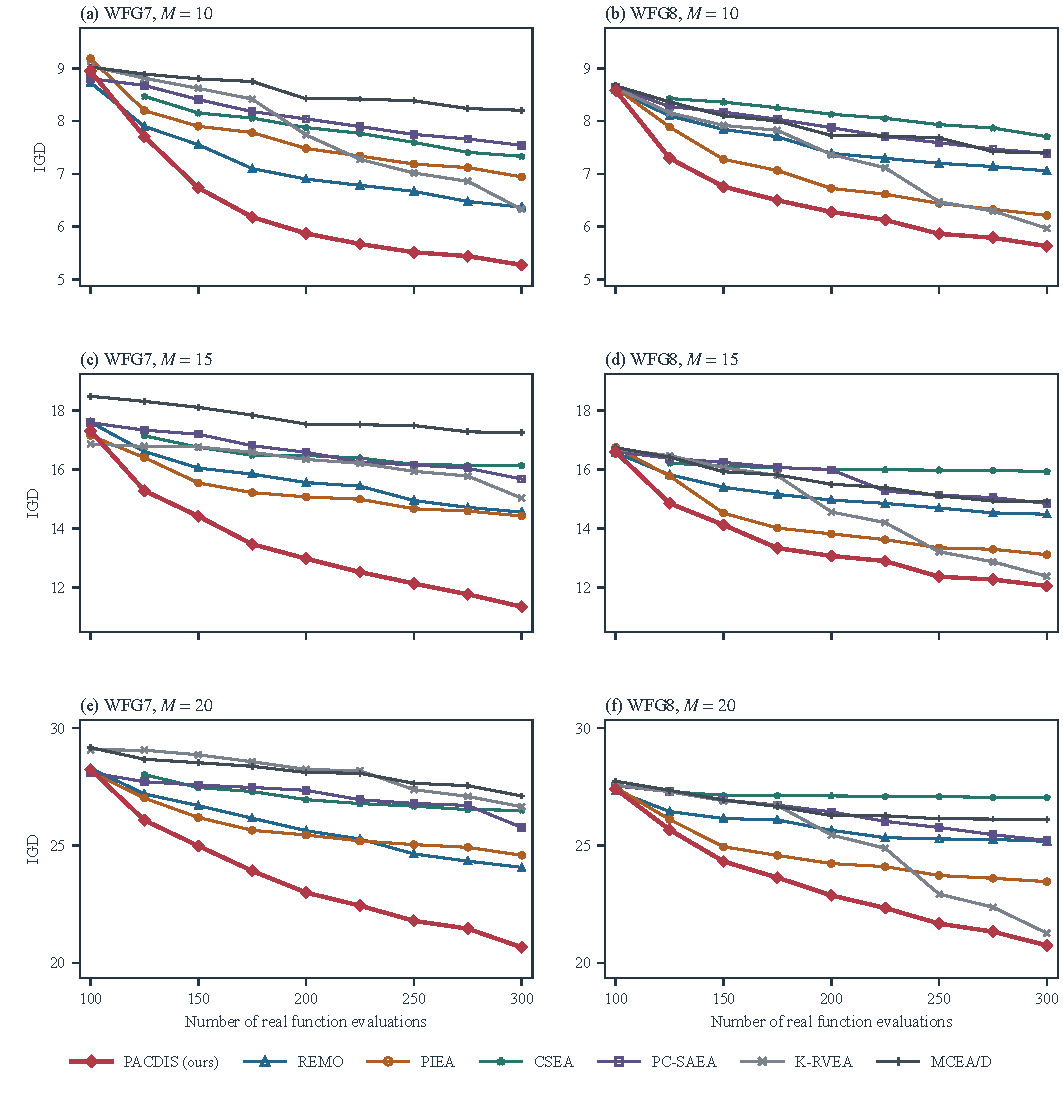
\includegraphics[width=0.98\textwidth]{figures/fig_convergence.pdf}
  \caption{Median IGD convergence of PACDIS and the six baseline algorithms
  on WFG7 and WFG8 at $M=10$, 15 and 20. Each curve summarizes 20
  independent runs (run identifiers 1--20) of the same experiment as the
  main comparison and starts at the algorithm's first recorded snapshot,
  because the initial design already consumes real evaluations. Traces are
  aligned on a unit-FE grid by holding the most recent recorded value,
  without extrapolation past the last snapshot, and one vertex is drawn
  every 25 evaluations. The IGD values are computed by the same
  implementation and reference sets as
  Tables~\ref{tab:exp:dtlz} and~\ref{tab:exp:wfg}.}
  \label{fig:exp:convergence}
\end{figure*}


\subsection{Effect of Selection-Criterion Switching}
\label{sec:exp:pmix}

Equation~\eqref{eq:mode} retains $p_{\mathrm{mix}}=0.5$ as the default.
The existing five-setting sensitivity experiment uses Lambdat030 with batch
distance and IGD. Its rankings do not establish a preferred setting for
NoBatchDist under IGD$^+$.
\TODO{Evaluate the two endpoint settings, $p_{\mathrm{mix}}=0$ and 1,
against the default on the same six problems at $M=10$ and 20.
Reuse default runs only after checking their protocol. Reuse old endpoint
runs only with evidence that every executed selection path is equivalent;
$p_{\mathrm{mix}}=1$ still permits exploration when the indicator model fails.}

\subsection{Convergence Behavior}
\label{sec:exp:convergence}

Figure~\ref{fig:exp:convergence} uses the cached IGD$^+$ trajectories of
NoBatchDist and the six baselines on WFG7 and WFG8. The source files match
the main-table run identifiers 1--20. We retain the earlier choice of
problems to keep the figure's scope fixed during the version update.

The horizontal axis counts actual evaluations, including initialization.
We align snapshots on a unit-FE grid using the latest recorded value at or
before each grid point, and draw vertices every 25 evaluations up to 300.
The display starts at 95 and does not extend traces beyond their last
snapshot. For runs that finish after 300 evaluations, the value at 300
comes from the latest snapshot within the budget; it can differ from the
terminal value in the main table.

At 300 evaluations, PACDIS has the lowest median IGD$^+$ in five of the
six panels. K-RVEA has the lowest median on WFG8 at $M=20$
(17.736 versus 17.981 for PACDIS). Thus, the mean-based advantage in the
main tables does not imply the lowest median in every panel.


% Experimental floats are queued early enough to precede the conclusion.
\section{Conclusion}
\label{sec:conclusion}
PAQC supplements REMO's representative-based grouping with PBI-based quality information
from directions constructed directly from the current nondominated set.
The motivation is that representatives selected through a two-dimensional
radial grid may not fully reflect the distribution in the original
high-dimensional objective space. PAQC combines the two information sources to form
the positive training group, while CDIS supports batch selection under a limited
evaluation budget.

\TODO{ State the strongest verified algorithm-level
result and its benchmark scope. Close by connecting the group-composition and
candidate-batch findings to these two design roles, keeping empirical performance
claims at the level supported by their matched comparisons.}

\begin{thebibliography}{99}

\bibitem{ref:moead}
Q.~Zhang and H.~Li,
``MOEA/D: A multiobjective evolutionary algorithm based on decomposition,''
\emph{IEEE Trans. Evol. Comput.}, vol.~11, no.~6, pp.~712--731, 2007.

\bibitem{ref:remo}
H.~Hao, A.~Zhou, H.~Qian, and H.~Zhang,
``Expensive multiobjective optimization by relation learning and prediction,''
\emph{IEEE Trans. Evol. Comput.}, vol.~26, no.~5, pp.~1157--1170, 2022.

\bibitem{ref:rsea}
C.~He, Y.~Tian, Y.~Jin, X.~Zhang, and L.~Pan,
``A radial space division based evolutionary algorithm for many-objective
optimization,'' \emph{Applied Soft Computing}, vol.~61, pp.~603--621, 2017.
\href{https://doi.org/10.1016/j.asoc.2017.08.024}{doi:10.1016/j.asoc.2017.08.024}.

\bibitem{ref:piea}
Y.~Li, W.~Li, S.~Li, and Y.~Zhao,
``A performance indicator-based evolutionary algorithm for expensive
high-dimensional multi-/many-objective optimization,''
\emph{Information Sciences}, vol.~678, art.~121045, 2024.

\bibitem{ref:sde}
M.~Li, S.~Yang, and X.~Liu,
``Shift-based density estimation for Pareto-based algorithms in
many-objective optimization,''
\emph{IEEE Trans. Evol. Comput.}, vol.~18, no.~3, pp.~348--365, 2014.

\bibitem{ref:pcsaea}
Y.~Tian, J.~Hu, C.~He, H.~Ma, L.~Zhang, and X.~Zhang,
``A pairwise comparison based surrogate-assisted evolutionary algorithm for
expensive multi-objective optimization,''
\emph{Swarm Evol. Comput.}, vol.~80, art.~101323, 2023.

\bibitem{ref:csea}
L.~Pan, C.~He, Y.~Tian, H.~Wang, X.~Zhang, and Y.~Jin,
``A classification based surrogate-assisted evolutionary algorithm for
expensive many-objective optimization,''
\emph{IEEE Trans. Evol. Comput.}, vol.~23, no.~1, pp.~74--88, 2019.

\bibitem{ref:krvea}
T.~Chugh, Y.~Jin, K.~Miettinen, J.~Hakanen, and K.~Sindhya,
``A surrogate-assisted reference vector guided evolutionary algorithm for
computationally expensive many-objective optimization,''
\emph{IEEE Trans. Evol. Comput.}, vol.~22, no.~1, pp.~129--142, 2018.

\bibitem{ref:mcead}
T.~Sonoda and M.~Nakata,
``Multiple classifiers-assisted evolutionary algorithm based on decomposition
for high-dimensional multi-objective problems,''
\emph{IEEE Trans. Evol. Comput.}, vol.~26, no.~6, pp.~1581--1595, 2022.

\bibitem{ref:platemo}
Y.~Tian, R.~Cheng, X.~Zhang, and Y.~Jin,
``PlatEMO: A MATLAB platform for evolutionary multi-objective optimization,''
\emph{IEEE Comput. Intell. Mag.}, vol.~12, no.~4, pp.~73--87, 2017.

\end{thebibliography}

\end{document}
